\subsection{Testing the Questionnaire Language} \label{sec:TestingQL}

\subsubsection{Creating a Launch Configuration}

In order to test the language and the editor we need to deploy the developed
plugins within another Eclipse instance. For testing the easiest way is start a
so-called Runtime Instance.

Open the dialog \emph{Run / Run Configurations} and select the node \emph{Eclipse
Application} from the left tree widget and press the icon with the +
sign to create a new Launch Config.

You could leave the defaults here or change the name and location like in the
screenshot.

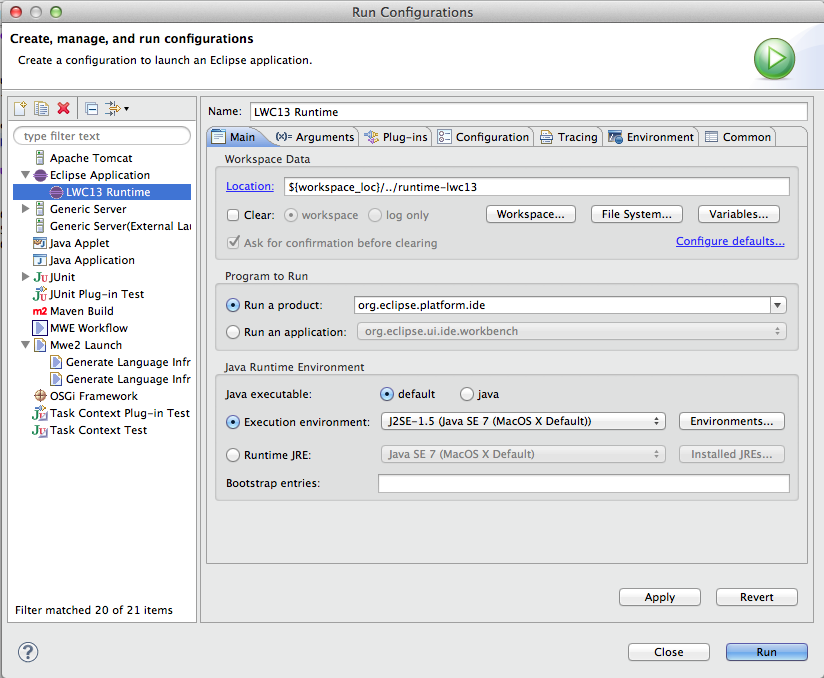
\includegraphics[width=17cm]{./images/chapter01/LaunchConfig.png}

Now switch to the Arguments page and enter in the ``VM arguments'' text box:
\begin{lstlisting}
-Xms40m -Xmx512m -XX:MaxPermSize=150m
\end{lstlisting}
Especially important is the MaxPermSize setting, since the default size of the
PermGen space of the VM (64MB) often is not enough.

Now press the \emph{``Run''} button. Another Eclipse instance will start with an
empty workspace. Close the Welcome window.


\subsubsection{Create Test Project}

In the Runtime Workspace create a new Plug-in Project with name
``QLTest''.\footnote{As before, uncheck the options on the second wizard page.}

First, we will create a dependency to the library plugin. Open the
\texttt{META-INF/MANIFEST.MF} file and switch to page Dependencies. In the \emph{Required
Plug-ins} section, add a dependency to \texttt{org.eclipse.xtext.example.ql.lib}.

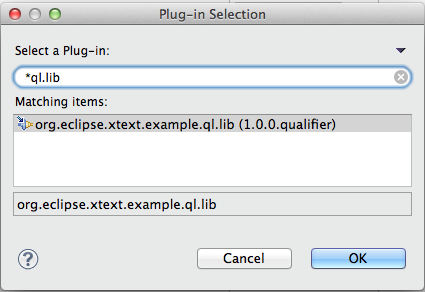
\includegraphics[width=8cm]{./images/chapter01/AddDependency_01.png}

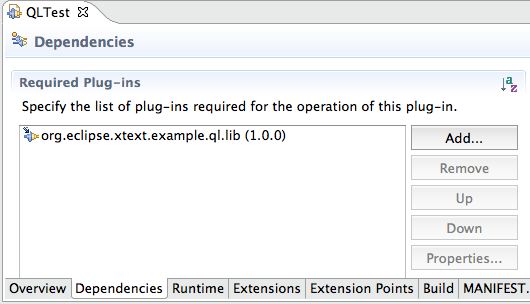
\includegraphics[width=10cm]{./images/chapter01/AddDependency_02.png}

The DSL has to support custom datatypes like \texttt{Money}, which must be
defined. Select the \texttt{/src} folder and create a new Java class \texttt{Money} in package
\texttt{types}:
\begin{lstlisting}[language=Java]
package types;

import java.math.BigDecimal;

public class Money {
  private BigDecimal amount;

  public Money(BigDecimal amount) {
    this.amount = amount;
  }

  public BigDecimal getAmount() {
    return amount;
  }
}
\end{lstlisting}
 

Select the \texttt{/src} folder and create a new file
\texttt{``housepurchase.ql''}. Once you have created the file a popup dialog
will appear to ask, if you would like to add the Xtext nature on this project.
Answer with ``Yes''.

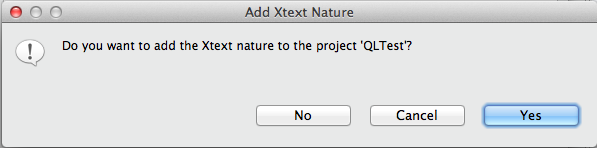
\includegraphics[width=12cm]{./images/chapter01/AddXtextNature.png}

From now on your project will be considered to contain files that Xtext should
recognize (\texttt{.ql} files). Projects having the Xtext nature will be processed by the
Xtext Builder when building projects, other projects are ignored. The Xtext
Builder indexes the Xtext based resources, links the cross-references in the
editor, and validates the model files. On errors, resource markers are created
which can be seen in the editor and the \emph{Problems View}.

Enter the content for
\texttt{``housepurchase.ql''}\footnote{\url{https://gist.github.com/kthoms/5036304}}:
\begin{lstlisting}[language=QL]
import types.Money

form Box1HouseOwning {
  hasSoldHouse: "Did you sell a house in 2010?" boolean
  hasBoughtHouse: "Did you by a house in 2010?" boolean
  hasMaintLoan: "Did you enter a loan for maintenance/reconstruction?" boolean

  sellingPrice: "Price the house was sold for    :" Money
  privateDebt: "Private debts for the sold house: " Money
  valueResidue: "Value residue: " Money
}
\end{lstlisting}

You see now that the editor has recognized our DSL. The language's keywords are
highlighted. Xtext offers far more than just syntax coloring for the language,
it created a fully integrated editor. You may explore some of the features now.

\begin{itemize}
  \item If you make errors, error markers are created and resolved while
you type.
\item Content assist is offered with CTRL+SPACE.
\item The Outline view \footnote{if not present, open with \emph{Window / Show View /
Outline}} presents the structure of the document, and allows quick navigation.
\item F3 allows jumping to the definition of an element, which is defined
somewhere else. You could try this by selecting ``Money'' and press F3. At the
moment, only the type information of questions is cross-referenced.
\end{itemize}

From now on, we will extend the DSL a bit further. This usually requires to
restart the test environment. So close it and proceed reading.
